% Depending on journal style:
%\renewcommand{\thepage}{S\arabic{page}}
%\renewcommand{\thesection}{S\arabic{section}}
\renewcommand{\thetable}{S\arabic{table}}
\setcounter{figure}{0}
\renewcommand{\thefigure}{S\arabic{figure}}

\section{Supplementary Materials}

\begin{figure*}[h!]
	\centering
	\begin{subfigure}[t]{0.48\textwidth}
		\centering
		\setlength{\fboxsep}{0pt}%
		\setlength{\fboxrule}{0.2pt}%
		\fbox{
			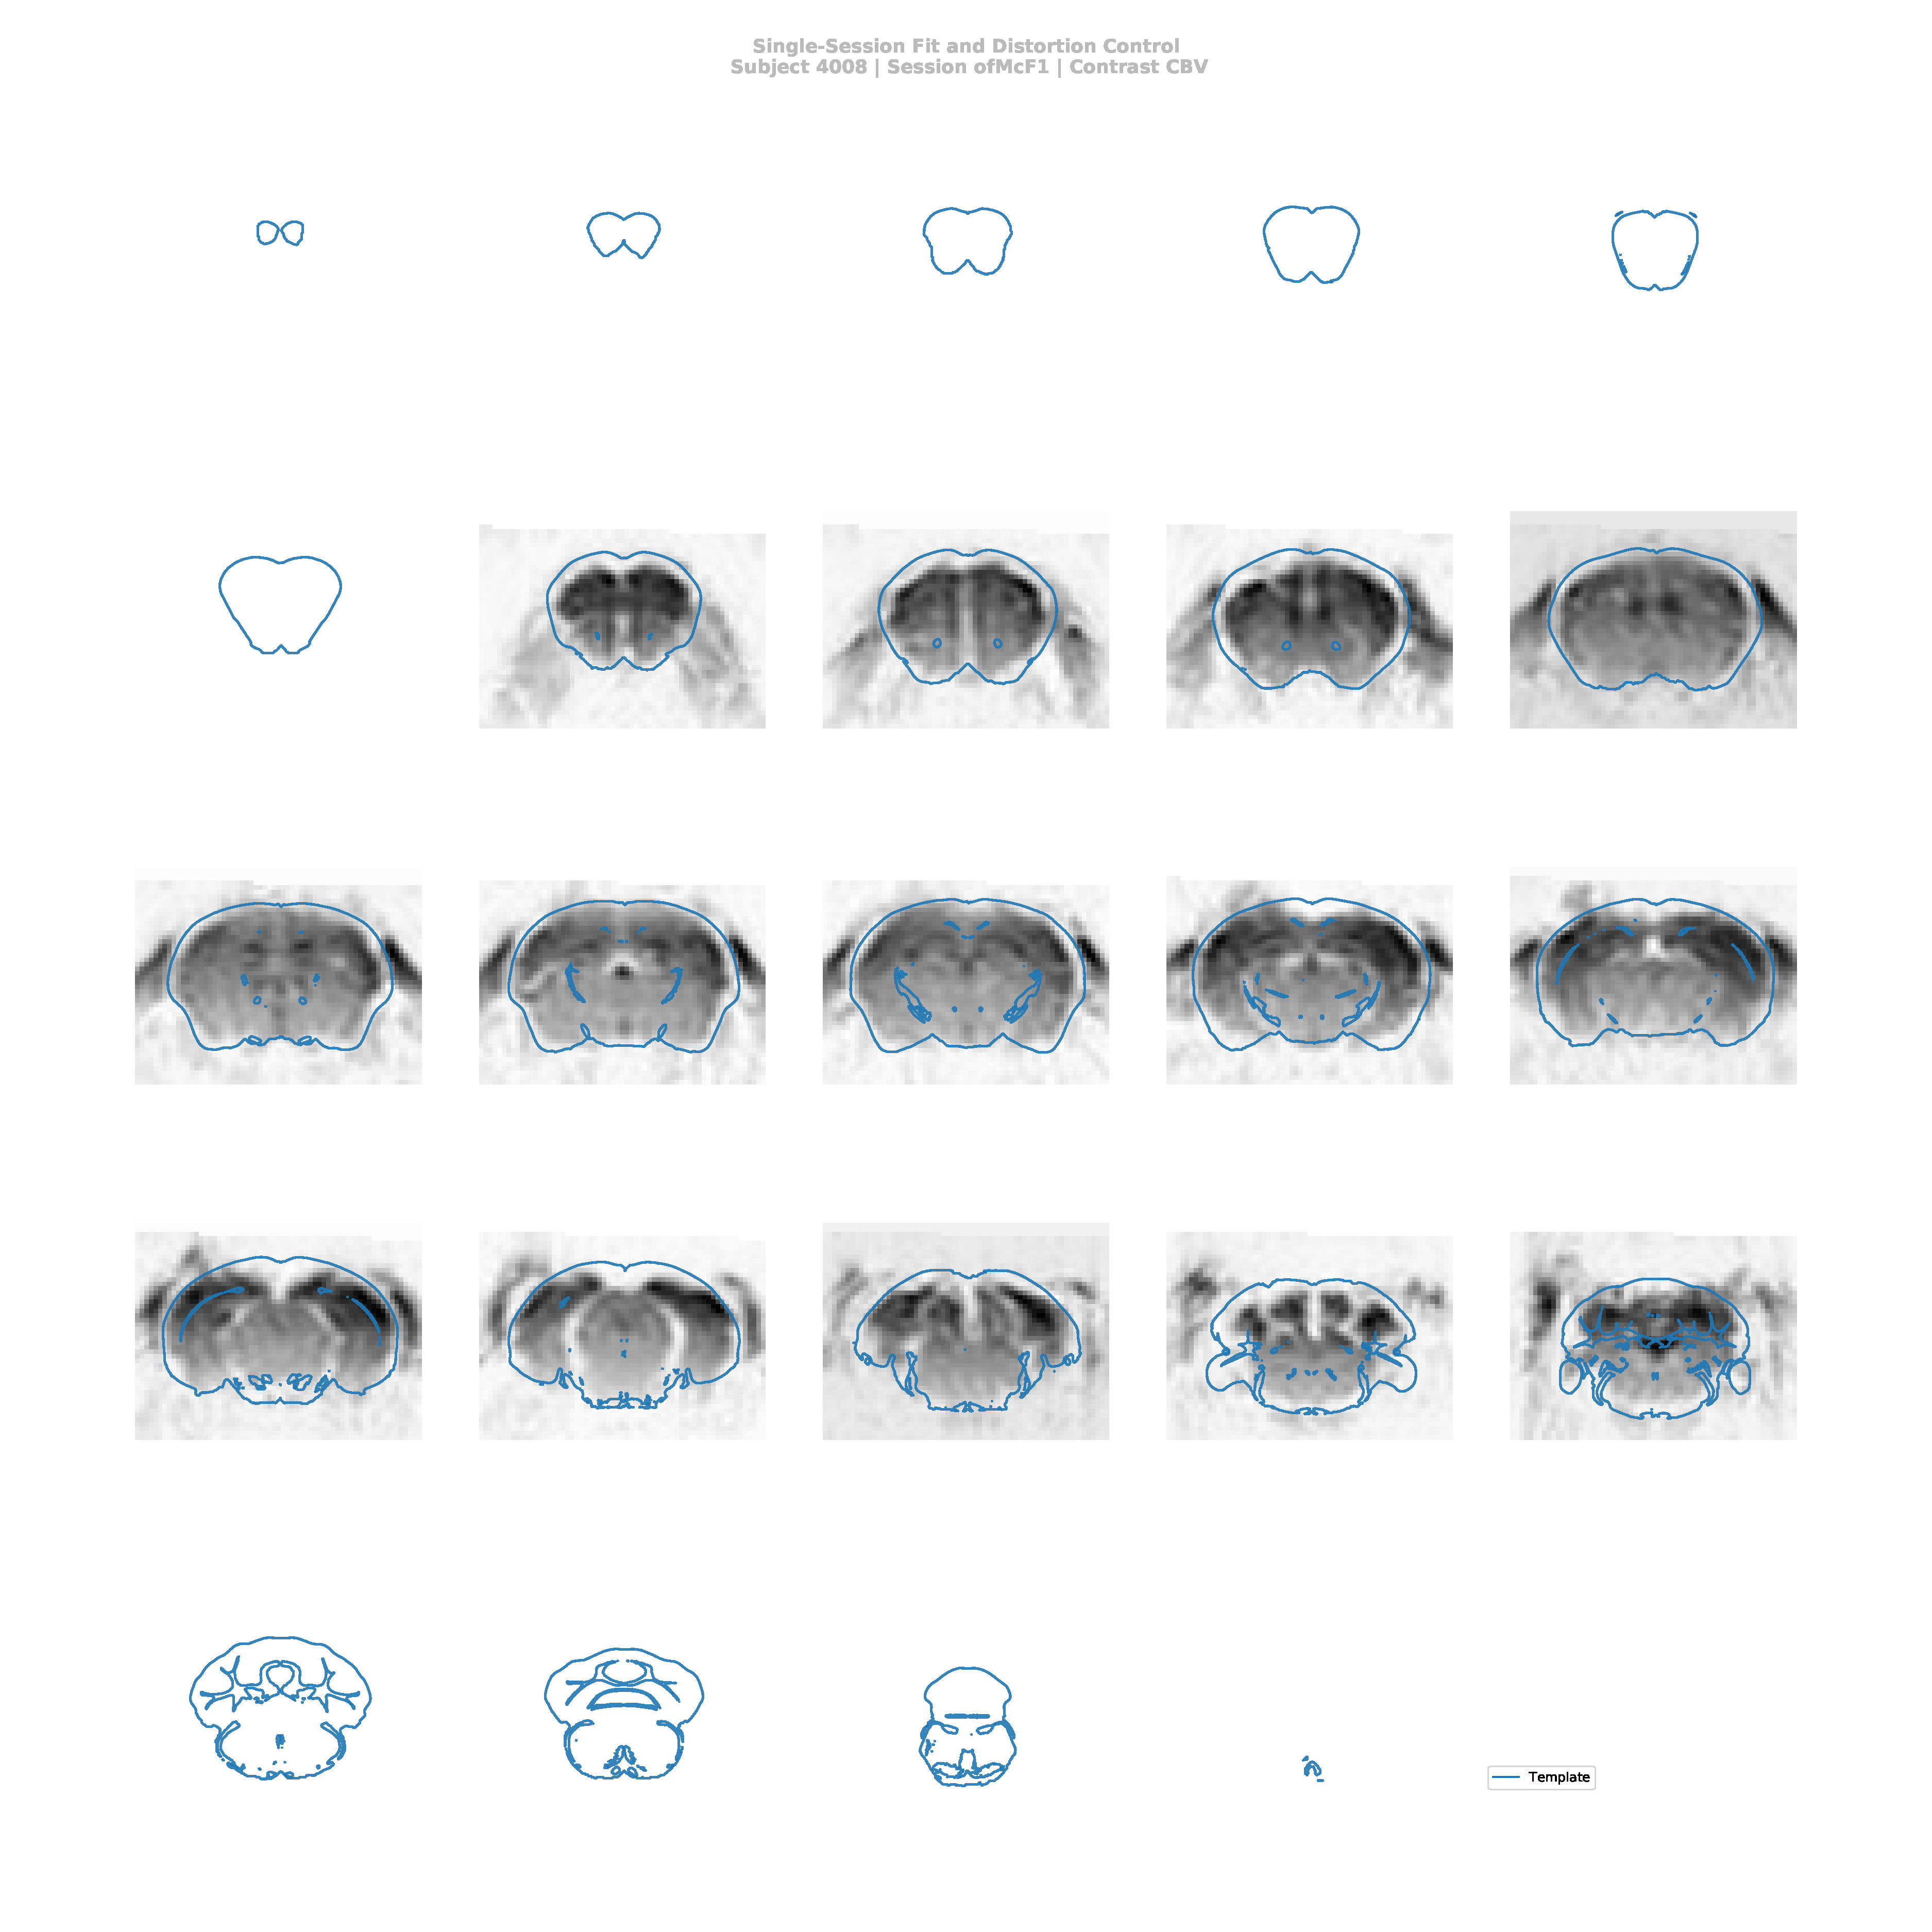
\includegraphics[width=\textwidth]{data/manual_overview/generic/4008_ofMcF1_cbv} 
			}
		\caption{
			SAMRI Generic workflow with Generic template, note the undistorted mapping and conservative smoothing.
			\vspace{1em}
			}
		\label{fig:fit_gg}
	\end{subfigure}\hfill
	\begin{subfigure}[t]{0.48\textwidth}
		\centering
		\setlength{\fboxsep}{0pt}%
		\setlength{\fboxrule}{0.2pt}%
		\fbox{
			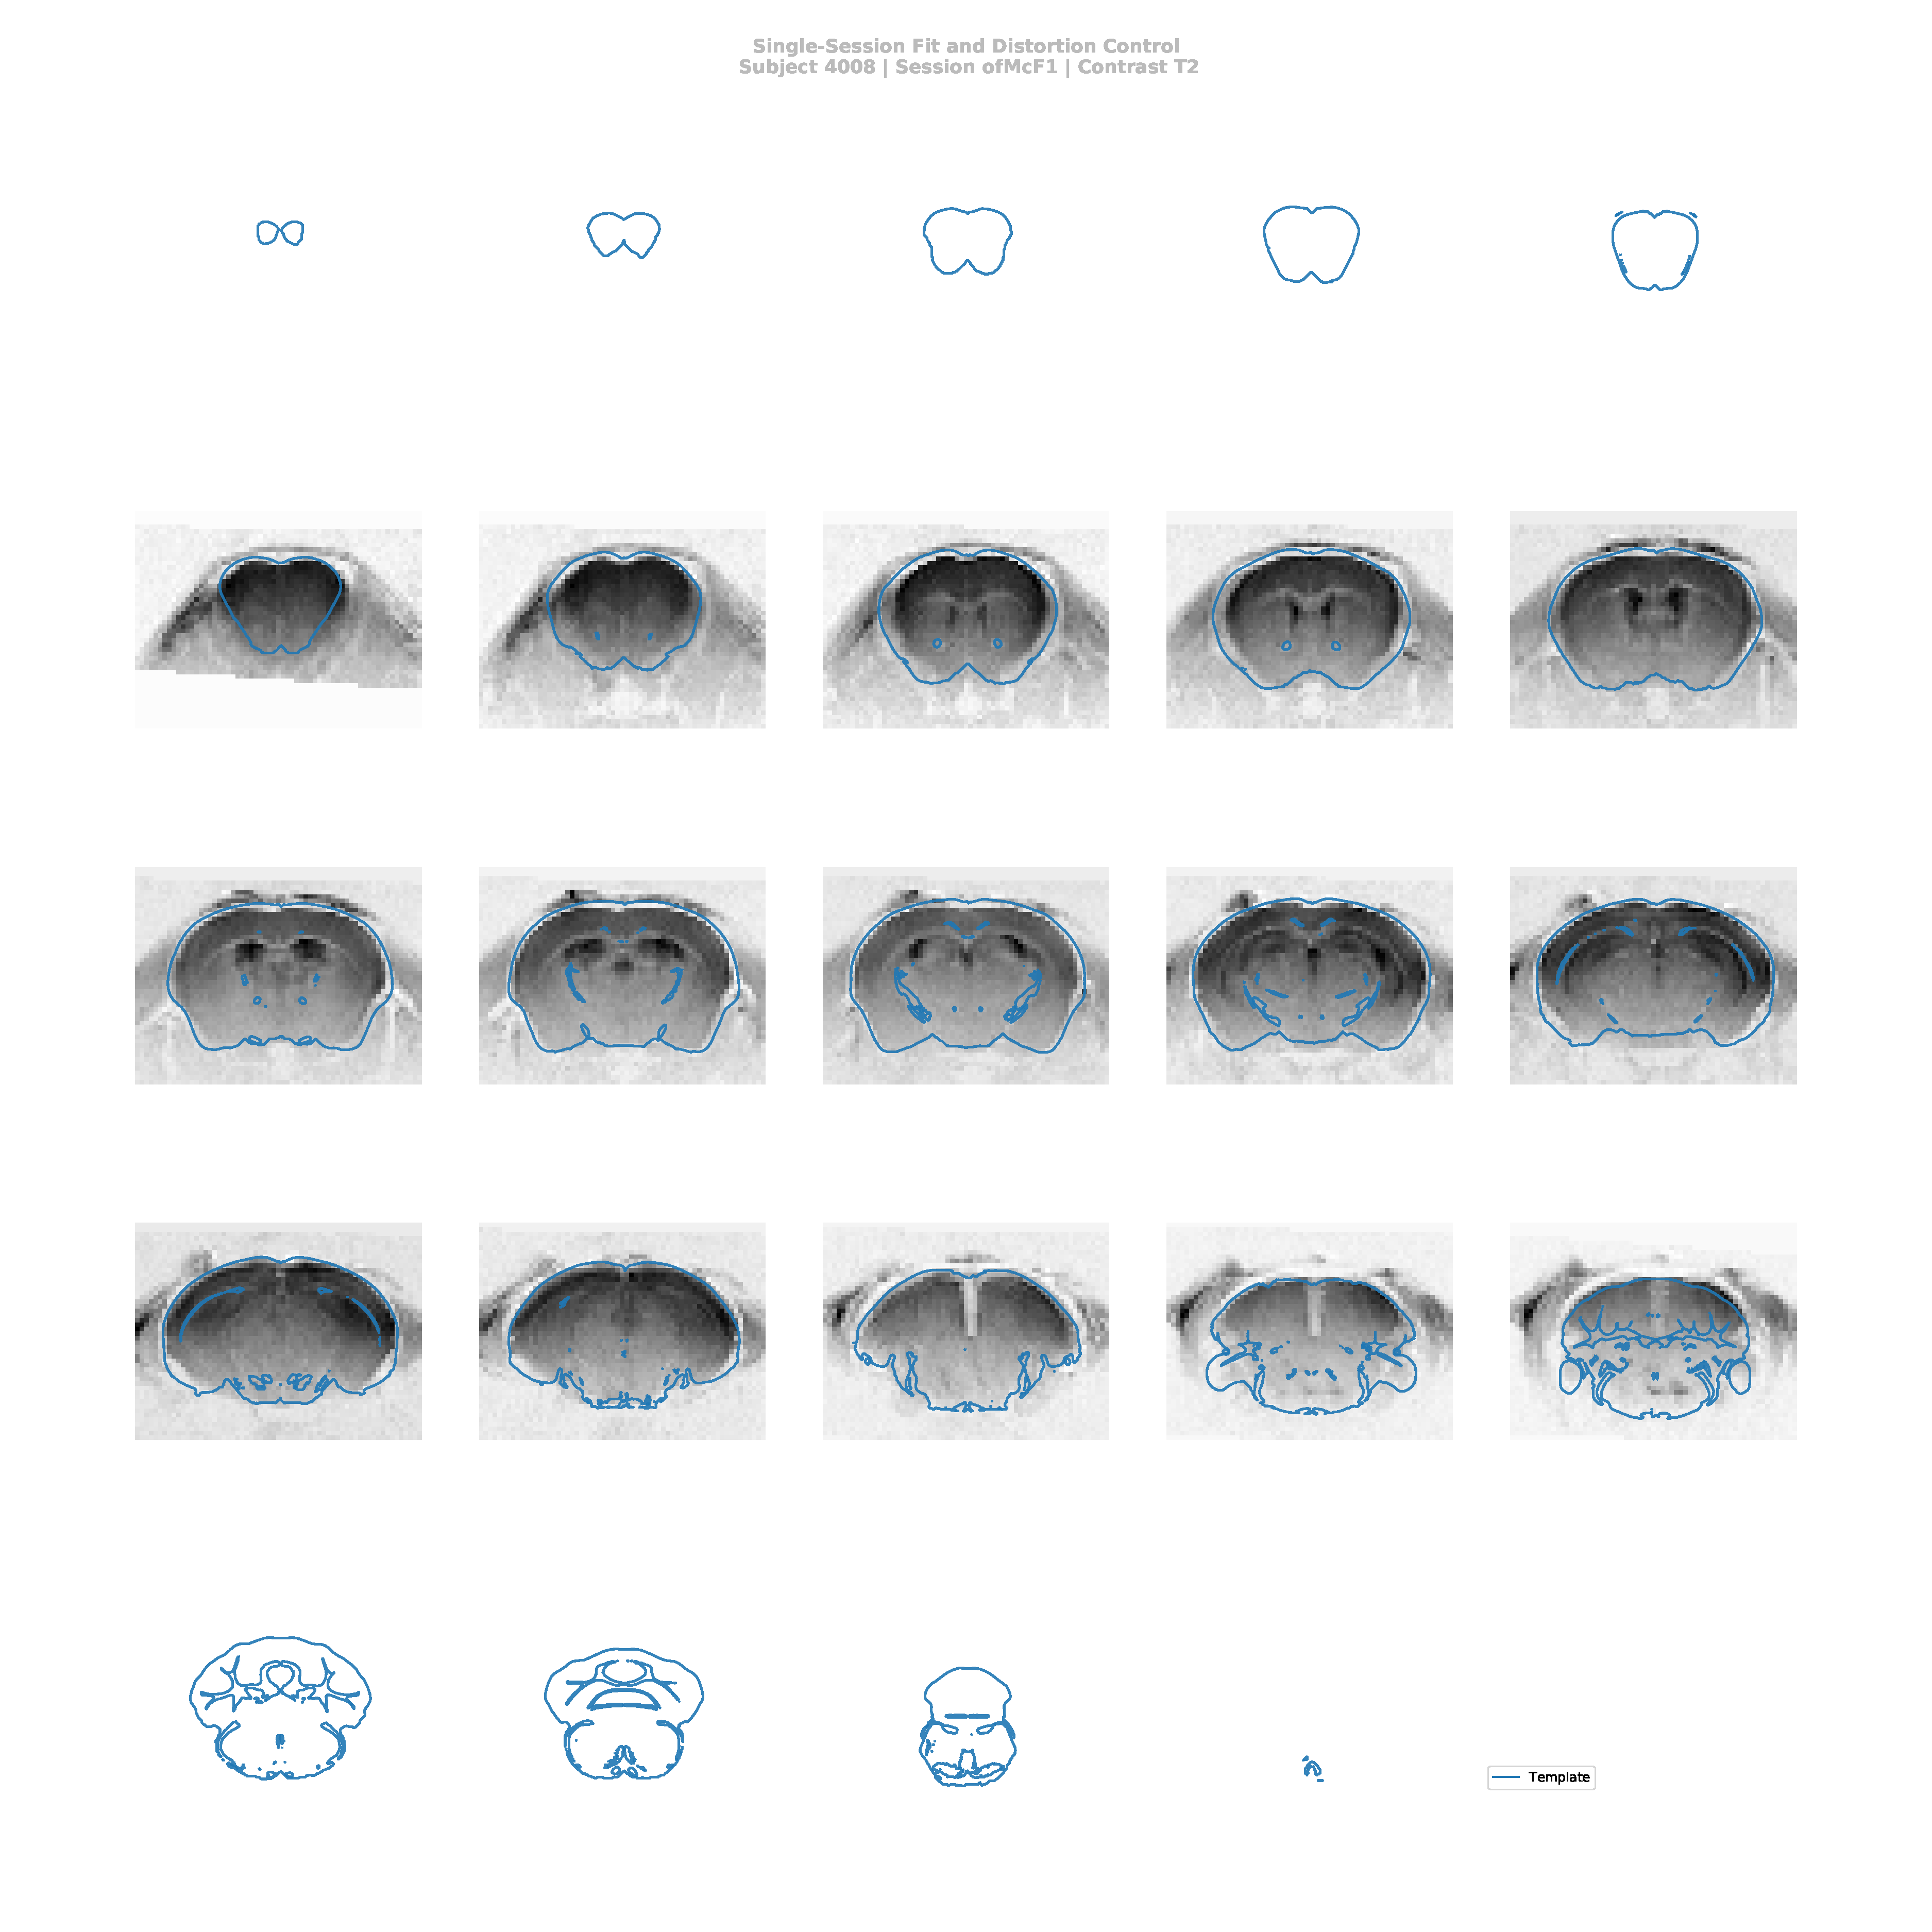
\includegraphics[width=\textwidth]{data/manual_overview/generic/4008_ofMcF1_T2w} 
			}
		\caption{
			SAMRI Generic workflow with Generic template, inspecting the structural scan intermediary; note the undistorted mapping and conservative smoothing.
			\vspace{1em}
			}
		\label{fig:fit_gga}
	\end{subfigure}
	\begin{subfigure}[t]{0.48\textwidth}
		\centering
		\setlength{\fboxsep}{0pt}%
		\setlength{\fboxrule}{0.2pt}%
		\fbox{
			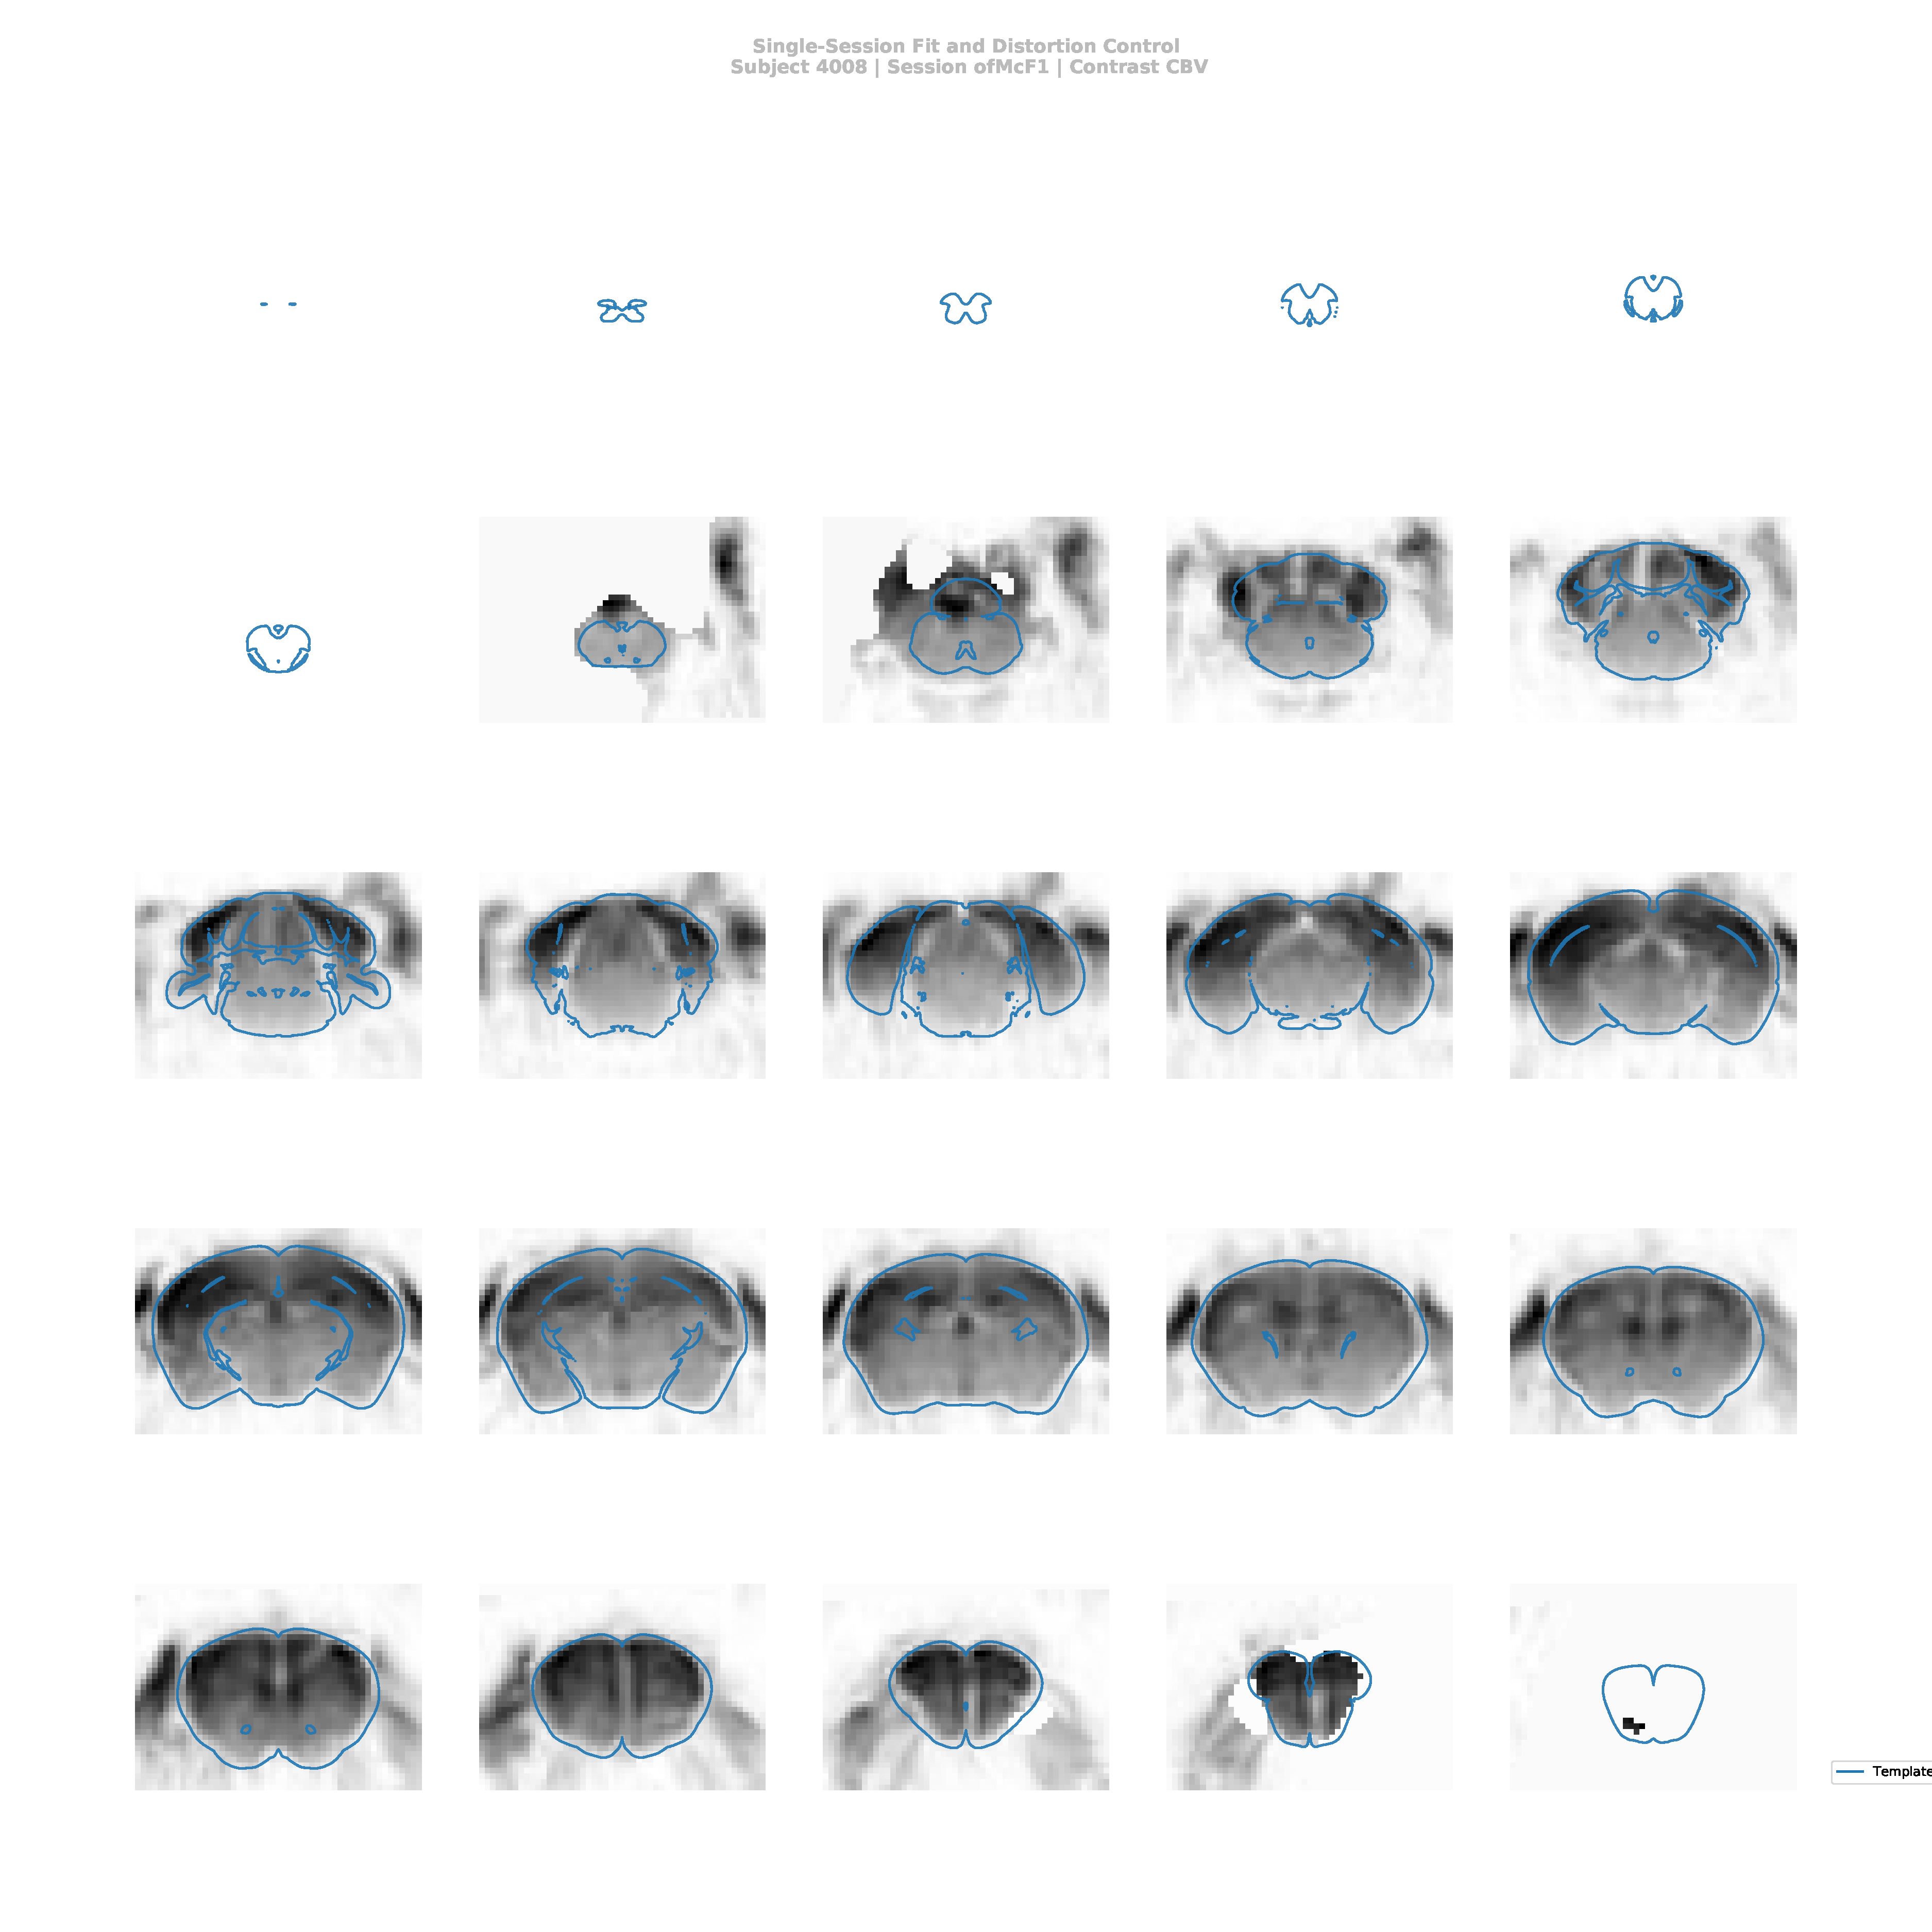
\includegraphics[width=\textwidth]{data/manual_overview/legacy/4008_ofMcF1_cbv} 
			}
		\caption{
			SAMRI Legacy workflow with Legacy template, note the strong smoothing and the mapping distortion in the rostral and caudal areas.
			}
		\label{fig:fit_ll}
	\end{subfigure}\hfill
	\begin{subfigure}[t]{0.48\textwidth}
		\centering
		\setlength{\fboxsep}{0pt}%
		\setlength{\fboxrule}{0.2pt}%
		\fbox{
			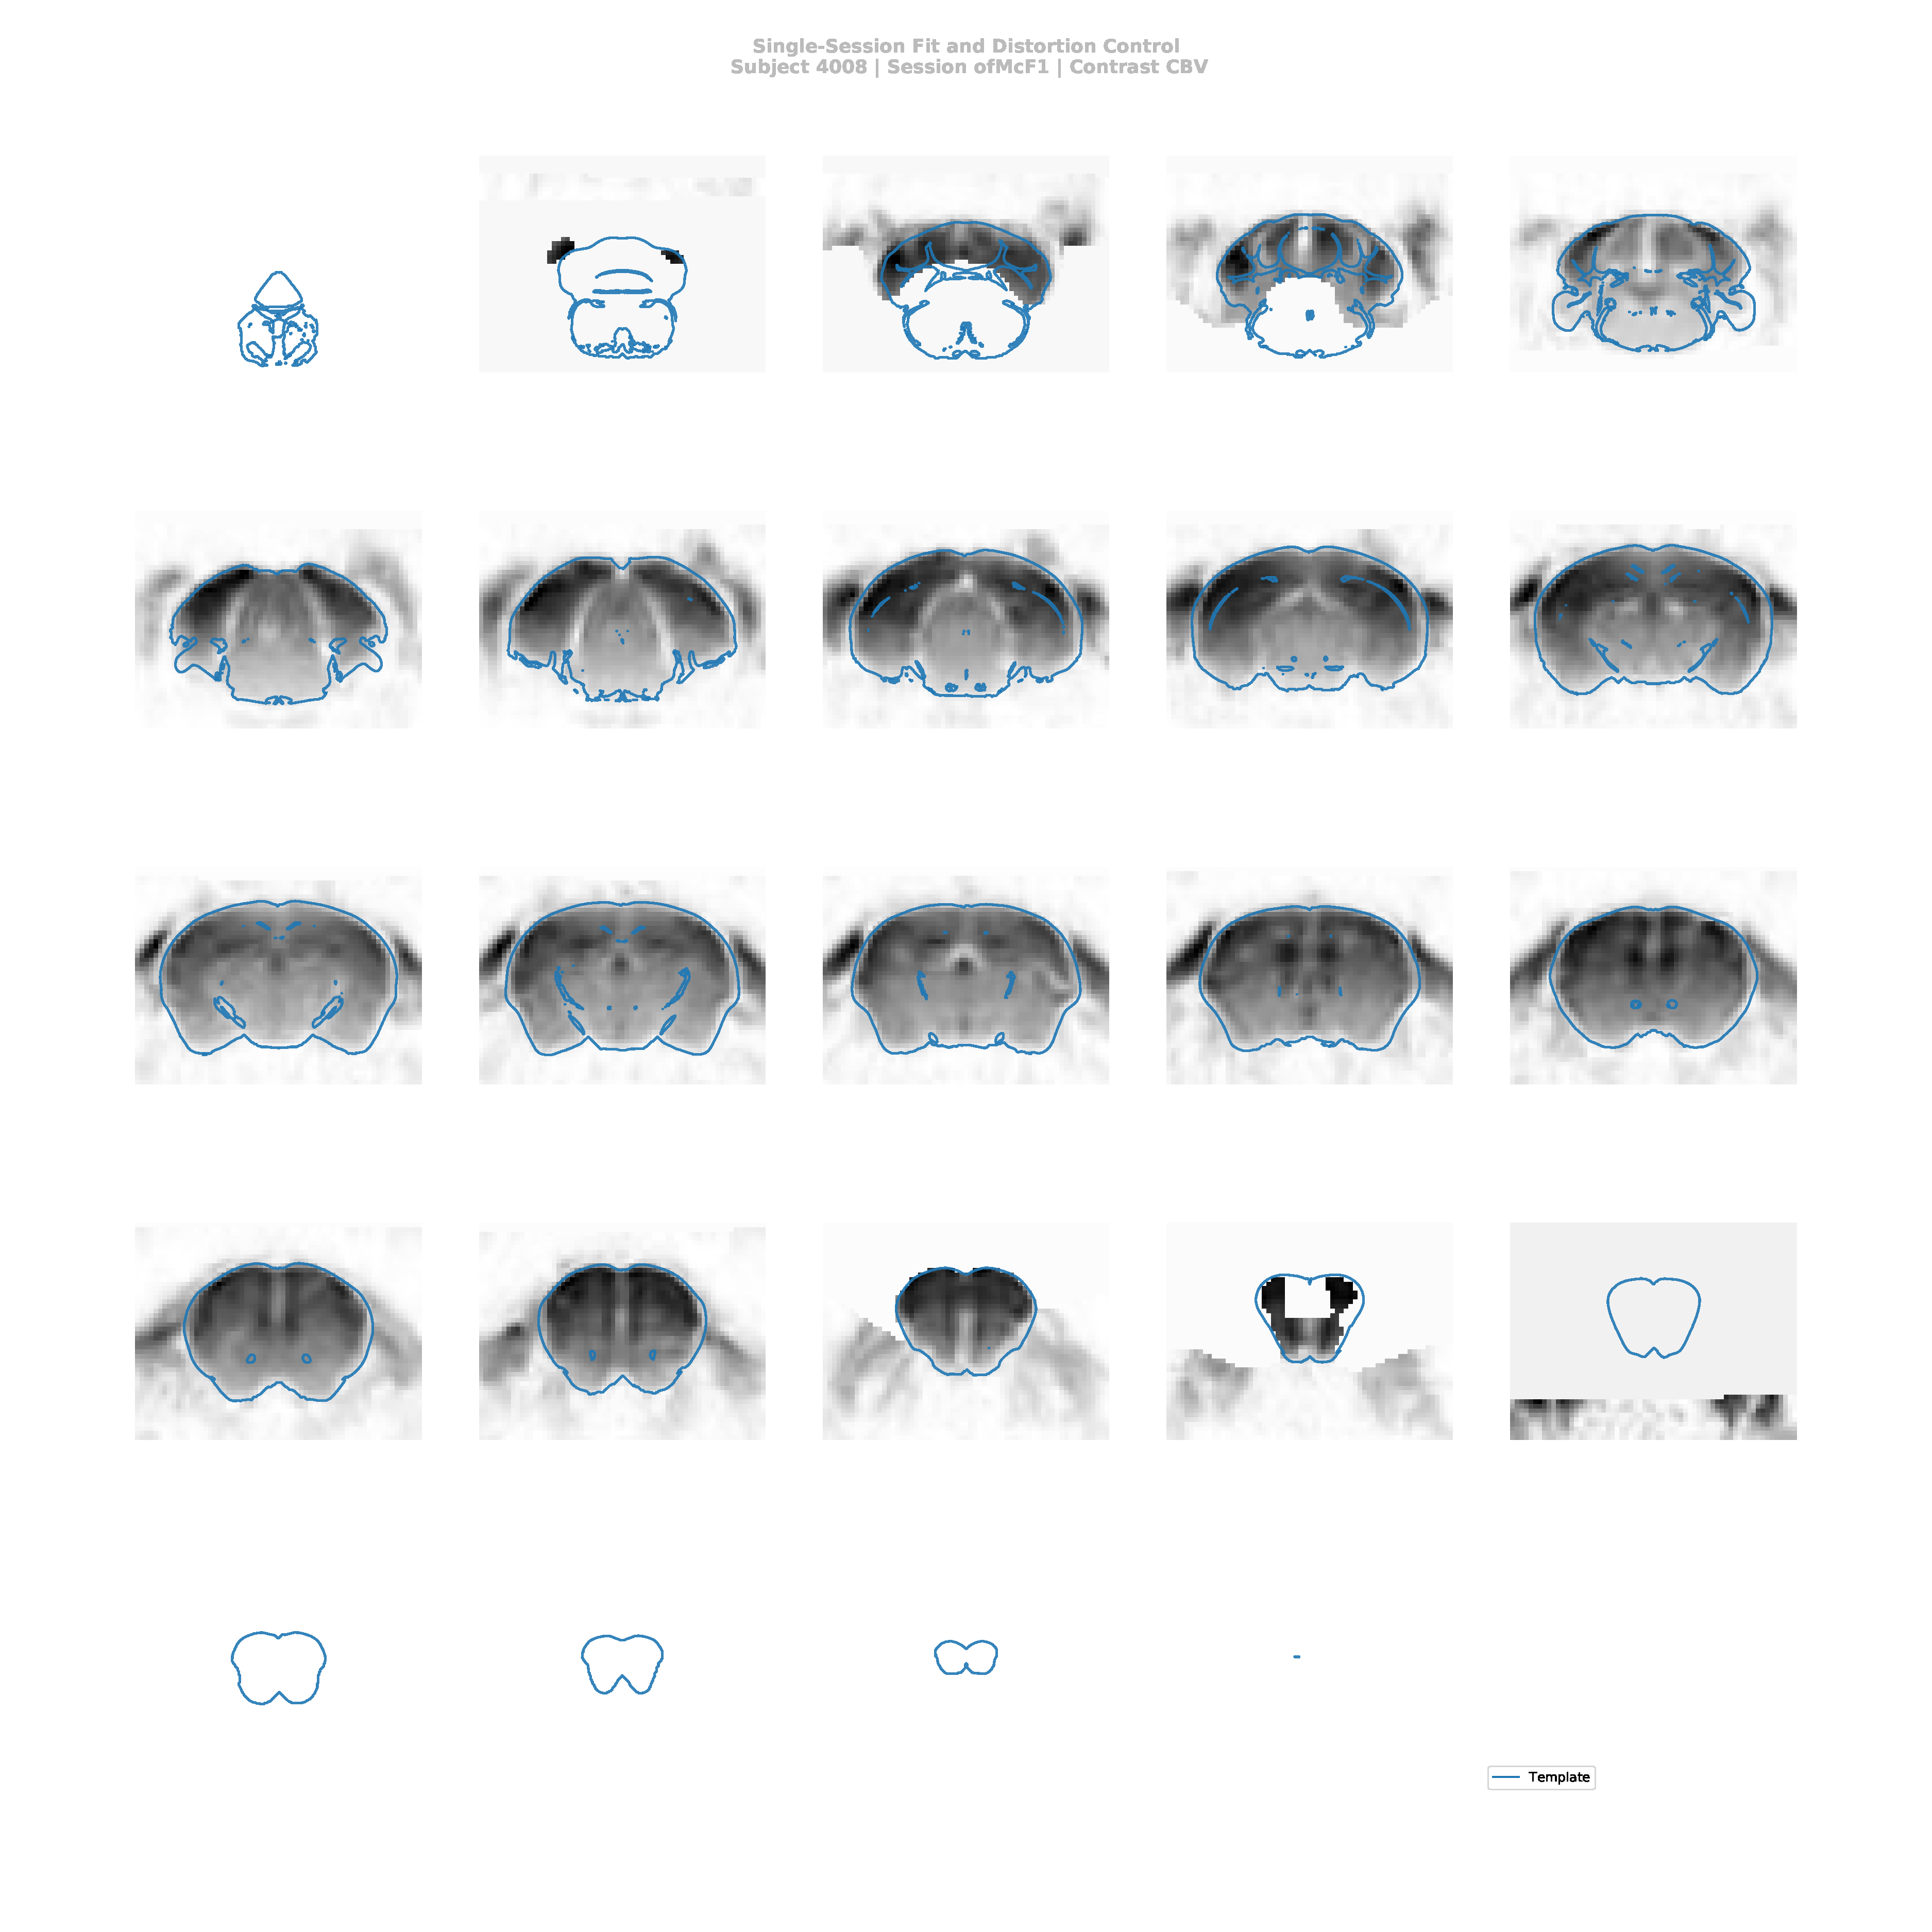
\includegraphics[width=\textwidth]{data/manual_overview/legacy_dsurqec/4008_ofMcF1_cbv} 
			}
		\caption{
			SAMRI Legacy workflow with Generic template, note the strong smoothing and the mapping distortion in the rostral and caudal areas.
			}
		\label{fig:fit_lg}
	\end{subfigure}
	\caption{
		\textbf{The SAMRI Generic workflow induces less smoothness, and provides more accurate coverage.}
		Depicted are automatically created operator overview graphics, which allow a slice-by-slice (spacing analogous to acquisition) inspection of the registration fit.
		This representation affords a particularly detailed view of the preprocessed MRI data, and highly accurate template contours.
		}
	\label{fig:fit}
\end{figure*}

\begin{figure*}[h!]
	\centering
	\setlength{\fboxsep}{0pt}%
	\setlength{\fboxrule}{0.2pt}%
	\fbox{
		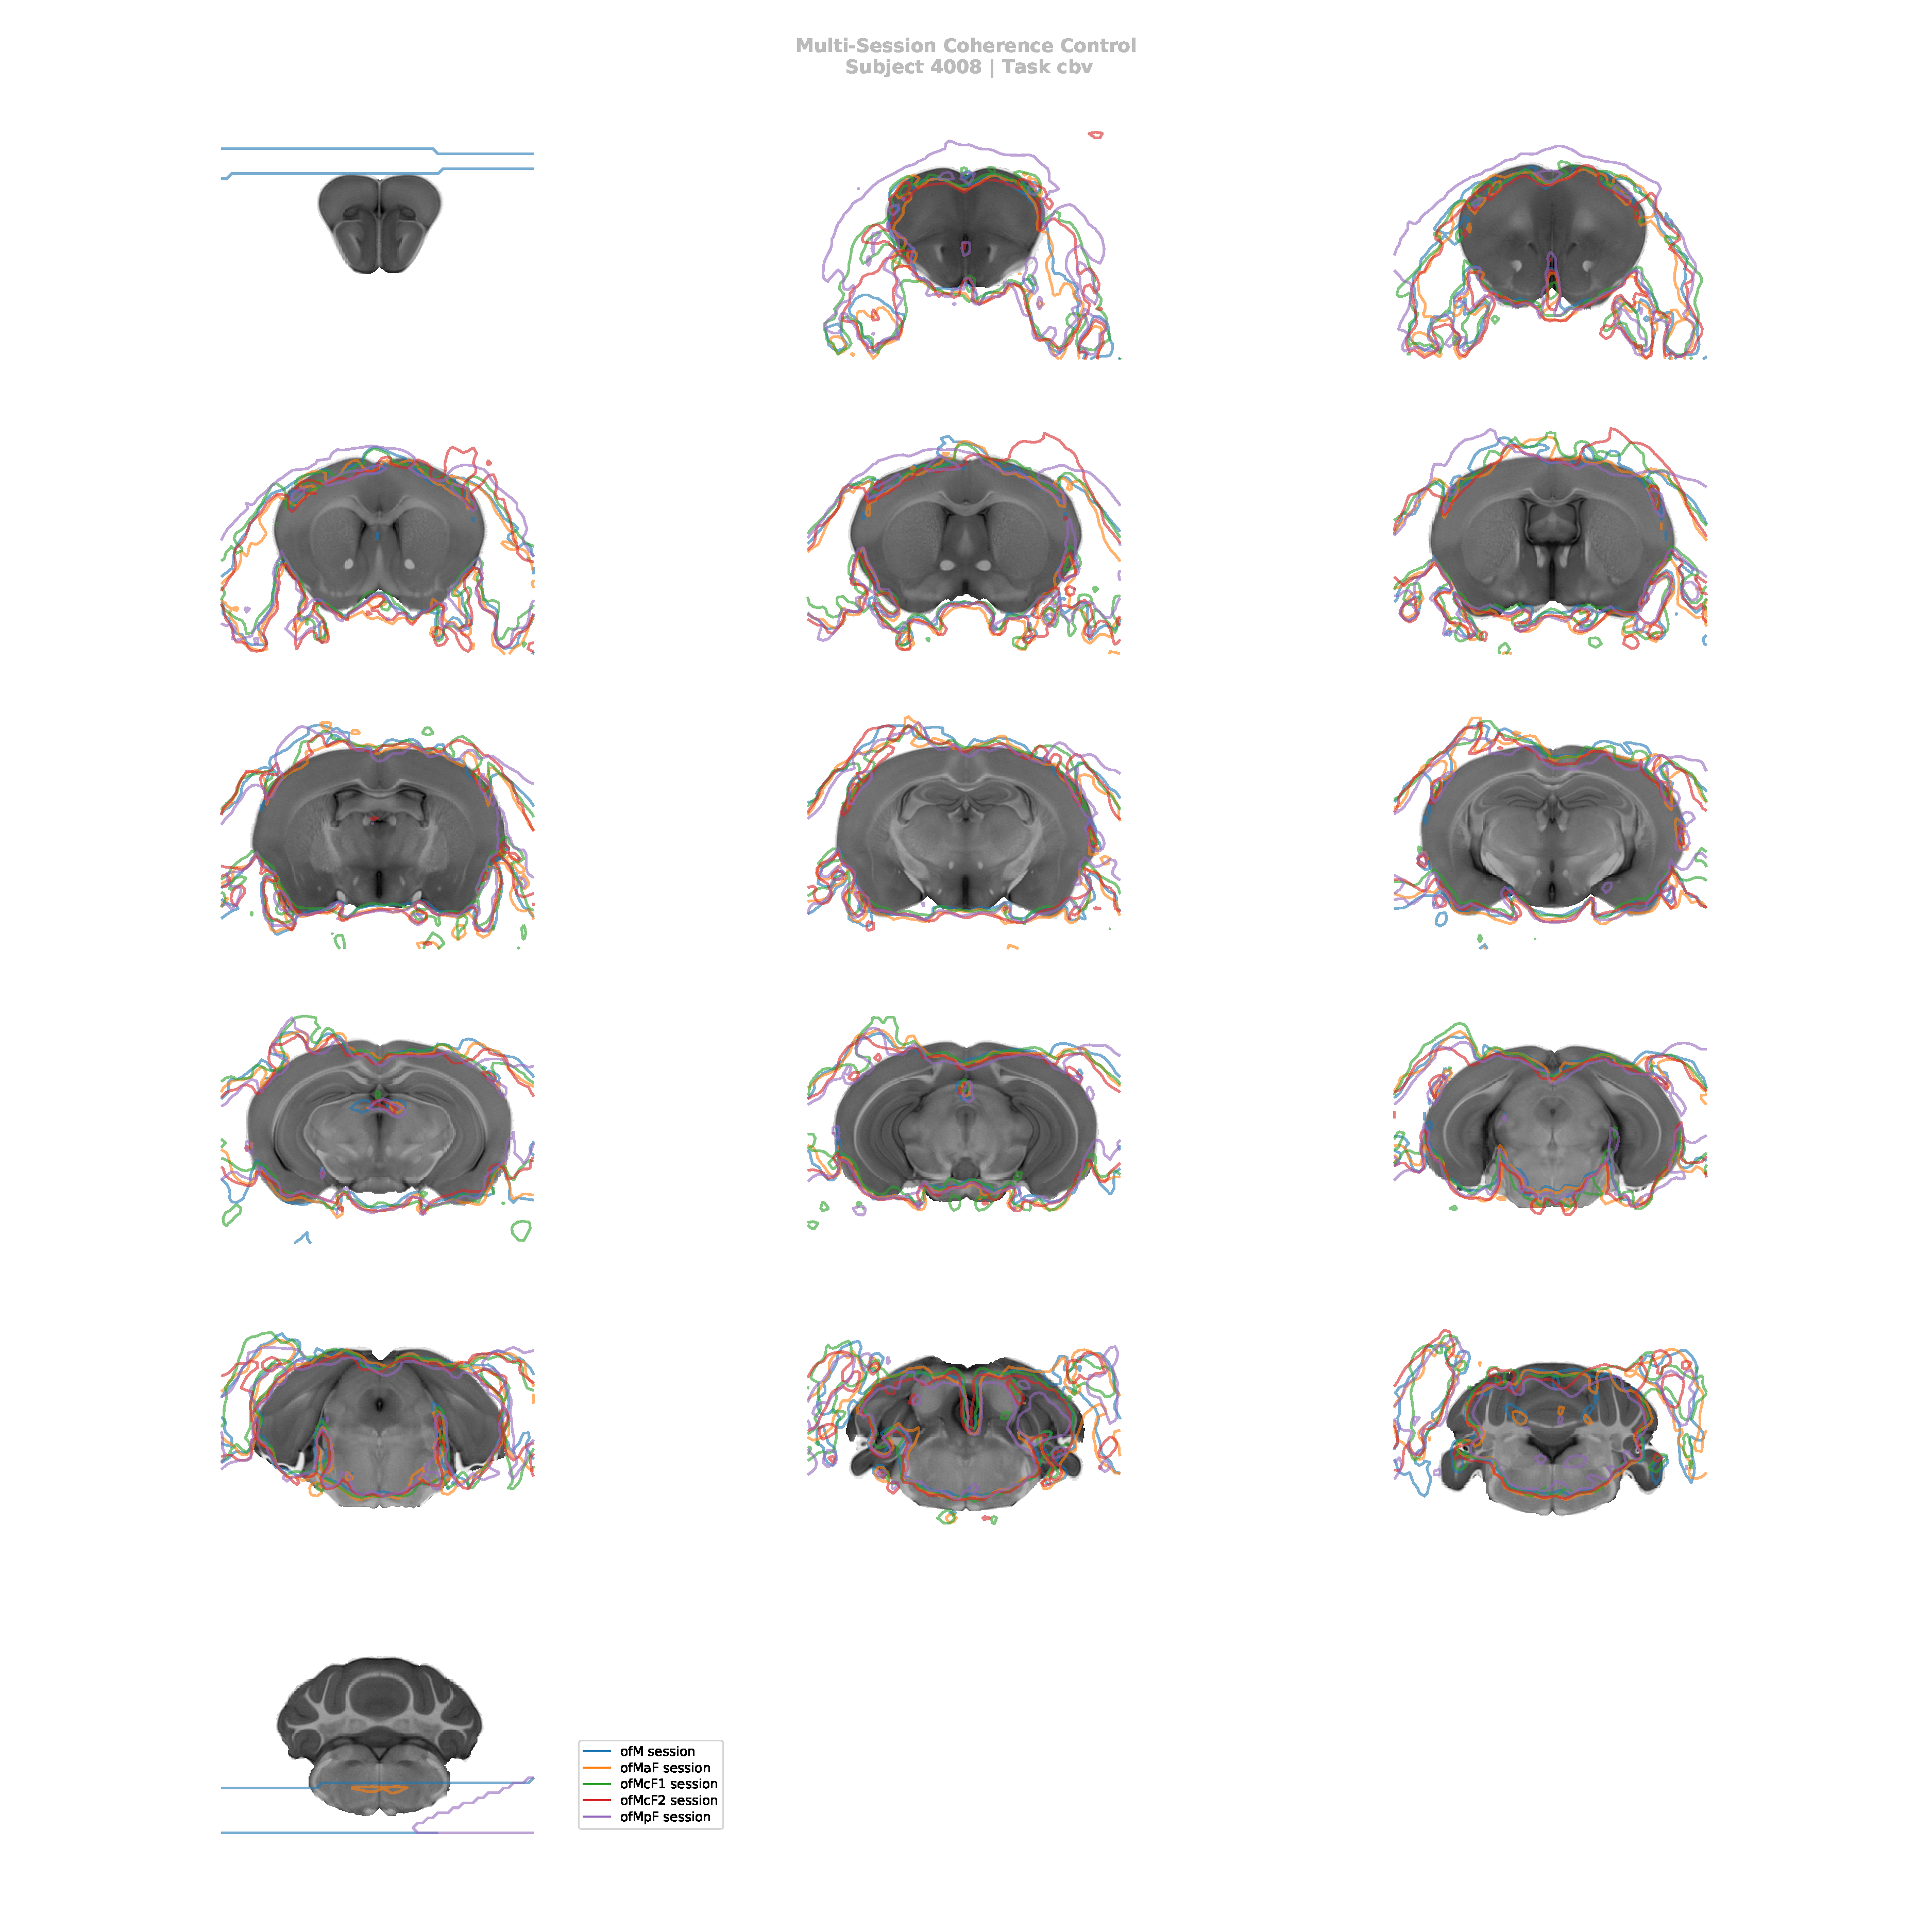
\includegraphics[width=\textwidth]{data/manual_overview/generic/coherence_4008_cbv} 
 		}
	\caption{
		\textbf{The SAMRI Generic workflow consistently maps high-salience features such as the implant site across sessions}
		Automatically created operator overview graphic, allowing a slice-by-slice (spacing analogous to acquisition) inspection of registration coherence.
		This representation permits a coarse assessment of registration consistency for multiple sessions --- though at the cost of some clarity.
		Particularly, this visualization, allows an operator to track the position of high-amplitude fixed features across scans in order to ascertain coherence (similarly to what is automatically assessed by the Variance analysis of the session factor).
		}
 	\label{fig:coherence}
\end{figure*}

\begin{figure*}[h!]
	\begin{subfigure}{.64\textwidth}
		\centering
		\includedot[width=\textwidth]{data/generic_nipype}
		\vspace{1.4em}
		\caption{
			“SAMRI Generic”  workflow, based on the \textcolor{mg}{\texttt{antsRegistration}} function.
			The pipeline uses a higher-resolution structural scan intermediary for registration (note the two processing streams), which facilitates differential handling of anatomical variation and susceptibility artefacts.
			The function used is highly parameterized, and both of its instances --- “s\niceus register” and “f\niceus register” --- are supplied in the workflow with defaults optimized for mouse brain registration.
			}
		\label{fig:nwfgg}
	\end{subfigure}\hfill
	\begin{subfigure}{.34\textwidth}
		\centering
		\includedot[width=\textwidth]{data/legacy_nipype}
		\vspace{-1.9em}
		\caption{
			“SAMRI Legacy” workflow, which is based on the \textcolor{mg}{\texttt{antsIntroduction.sh}} function (and other functions with hard-coded parameters optimized for human brain registration), and also performs destructive affine manipulations.
			}
		\label{fig:nwfgl}
	\end{subfigure}
	\caption{
		Directed acyclic graphs detailing the precise node names (as seen in the SAMRI source code) for the two alternate MRI registration workflows.
		The package correspondence of each processing node is appended in parentheses to the node name.
		The “utility” indication corresponds to nodes based on Python functions specific to the workflow, distributed alongside it, and dynamically wrapped via Nipype.
		The “extra\niceus interfaces” indication corresponds to nodes using explicitly defined Nipype-style interfaces, which are specific to the workflow and distributed alongside it.
		}
	\label{fig:nwfg}
\end{figure*}

\py{pytex_tab('scripts/stim_table.py',
                label='stim',
                caption='Stimulation protocol, as delivered during functional scans.
                        Stimulus event spacing and parameters are constant across scans, but the exact onset time is variable in the \SI{10}{\second} magnitude range due to scanner adjustment time variability.',
                options_pre='[htp] \\scriptsize \\centering \\resizebox{\\columnwidth}{!}{',
                data='data/JogB.tsv',
                options_post='}',
                )}

